\documentclass{article}
\usepackage{blindtext}
\usepackage{geometry}
 \geometry{
 a4paper,
 total={170mm,257mm},
 left=20mm,
 top=20mm,
 }
 
\usepackage{graphicx} % Required for inserting images

\title{PrepEmisSources \\ a framework for preparing volcanic emissions}
\author{Alexander Ukhov, Ibrahim Hoteit}
\date{KAUST, May 2025}

\begin{document}

\maketitle

\section{Introduction}
PrepEmisSources is a Python-based framework for preparing and visualizing atmospheric emission scenarios, particularly applicable to volcanic eruptions or similar emission events. It provides an infrastructure for defining vertical emission profiles with temporal and spatial resolution suitable for input into models like WRF-Chem (starting from v4.8). The framework employs a fully object-oriented design, leveraging inheritance and modular components to support multiple emission scenario types (e.g., continuous, pulsed, or time-varying eruptions). This modularity facilitates extensibility and reuse, enabling users to define custom scenario classes or integrate with external data sources from different studies [1,2]. PrepEmisSources supports visualization utilities for inspecting emission profiles/scenarios and diagnosing inputs before model execution.

\section{Dependencies}

scipy, netCDF4, xarray, matplotlib, pandas

\section{How to use}
The path to the WRF-Chem file with initial conditions ('wrfinput\_d01', for example) is required. Review the provided 'example*.py' files and modify them to suit your requirements. After the script execution, the necessary adjustments in the namelist.input file will be shown. For instance: \\ \\
    \&time\_control  \\
        auxinput13\_interval\_m = 10 \\
        frames\_per\_auxinput13 = 85 \\
        auxinput13\_inname     = 'wrfchemv\_d01.1991-06-15\_01:40:00' \\
    \&chem \\
        chem\_opt               = 402   \\
        emiss\_opt\_vol          = 3    \\ \\
These settings mean that the prepared emission file 'wrfchemv\_d01.1991-06-15\_01:40:00' will be read by WRF-Chem 85 times, starting from the moment when the model time passes '1991-06-15 01:40:00'. During the run, the WRF-Chem will read the data from the emission file at 10-minute intervals. Within each interval, the corresponding vertical distribution of emissions will be used.

\section{How to cite}
If you used this utility in your work, please do not forget to cite it as follows: 
Ukhov et al., Enhancing Volcanic Eruption Simulations with the WRF-Chem v4.8

\clearpage
\section{Class structure}
There are several base classes: VerticalProfile, EmissionScenario, WRFNetCDFWriter, Emission, and EmissionWriter. Their interconnections are shown in Figure \ref{fig1}. In most cases, the user is expected to adapt the example scripts. These examples cover the full capabilities of the utility.

\begin{figure}
    \centering
    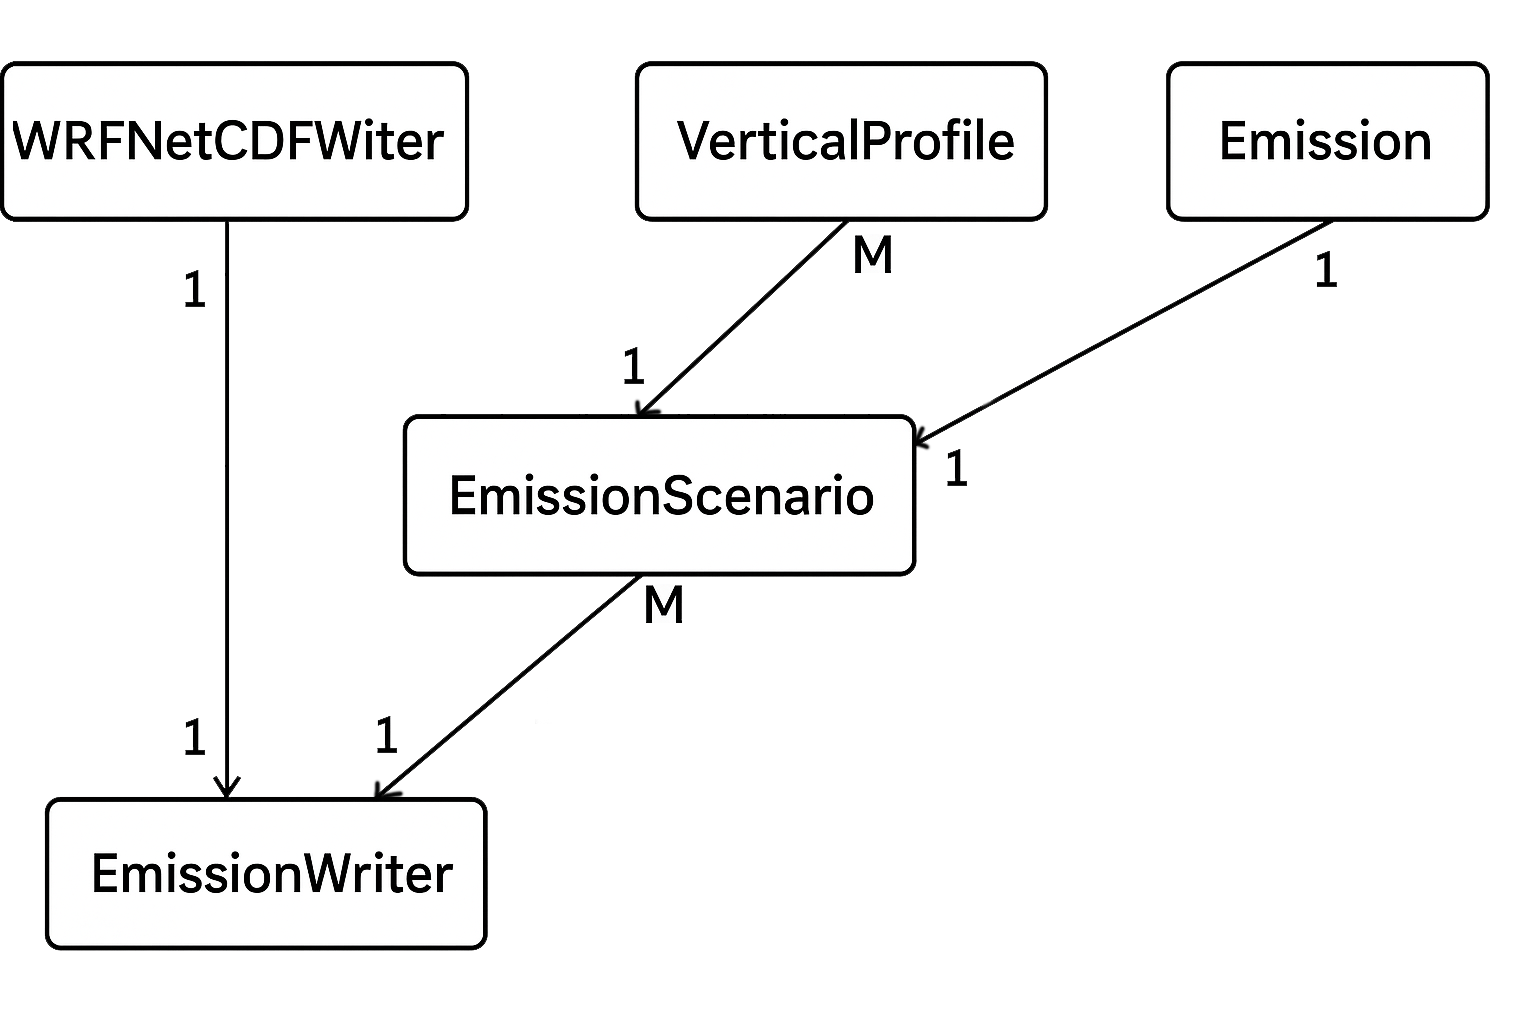
\includegraphics[width=0.7\linewidth]{./fig1_diagram.png}
    \caption{Base classes diagram. 1:1 arrows mean that one object is needed by another object (WRFNetCDFWriter and EmissionWriter objects, for example). 1:M means that many objects can be provided to encompass an object, i.e., EmissionScenario can comprise many vertical profiles.}
    \label{fig1}
\end{figure}

\subsection{VerticalProfile}
The emission profiles are managed through the `VerticalProfile` class, which maintains the height distribution and temporal information for each emission time step, enabling 4D (space and time) emission modeling. Each profile defines the mass flux distribution of emitted species across altitude levels at a given time step. The emitted mass in each profile can be scaled. Child classes are the following:

\subsubsection{VerticalProfile\_Zero}
A profile with zero emissions at all levels typically used to represent periods of inactivity.

\subsubsection{VerticalProfile\_Uniform}
A profile with a uniform emission distribution between specified minimum and maximum heights.

\subsubsection{VerticalProfile\_Umbrella}
A profile represents the umbrella-shaped distribution of volcanic eruptions, with parameters: maximum emission and vent heights and the percentage of mass in the 'umbrella' region.

\subsubsection{VerticalProfile\_Suzuki}
Based on [3] and [4], input parameters control the maximum emission height and 'skewness' of the umbrella.

Figure \ref{fig2} shows examples of different vertical profiles implemented in the PrepEmisSources utility.

\begin{figure}
    \centering
    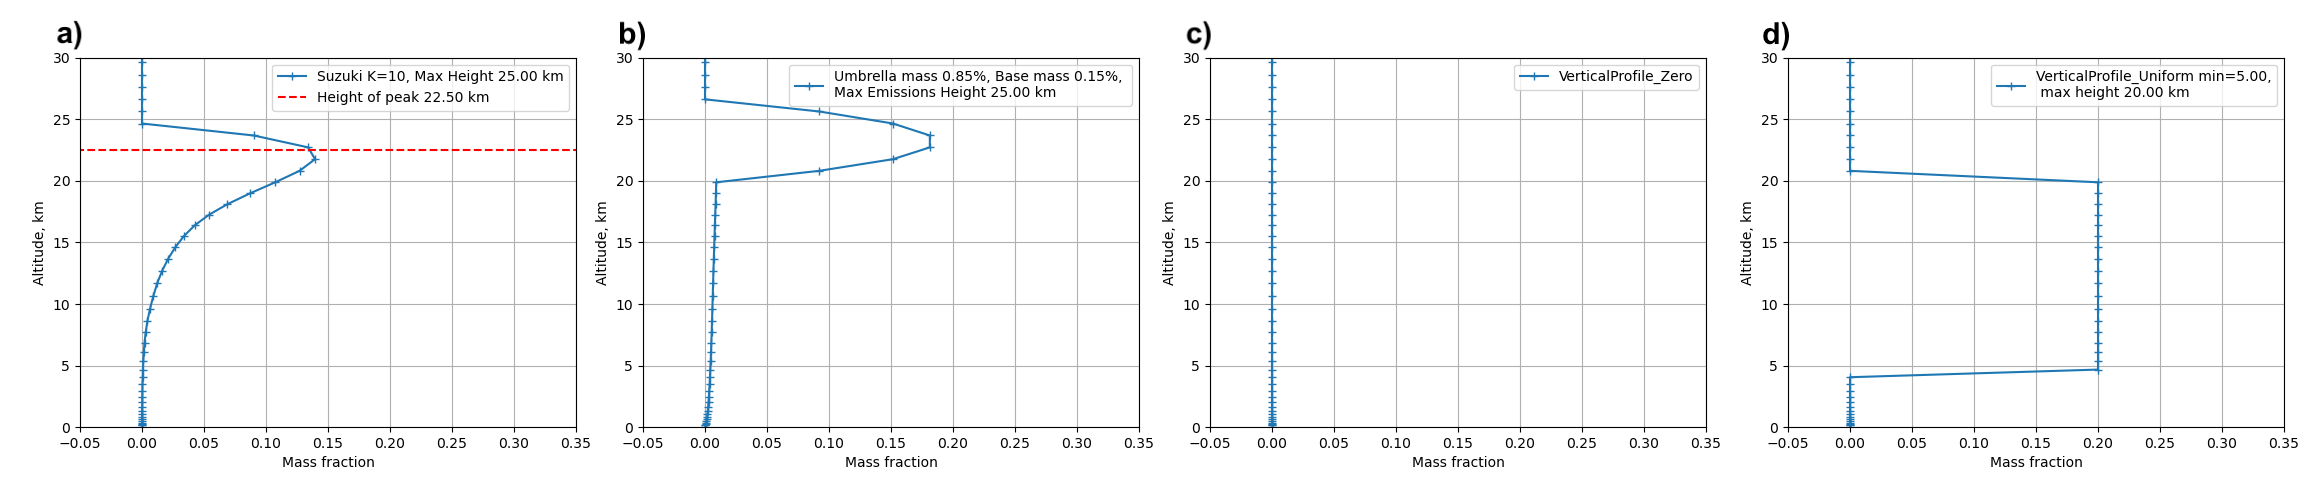
\includegraphics[width=1\linewidth]{fig2_profiles.png}
    \caption{Different vertical profiles, which define different ways to release the mass of volcanic material: a) Suzuki profile, b) Umbrella profile, c) Zero profile, d) Uniform profile.}
    \label{fig2}
\end{figure}

\subsection{Emission}
Base abstract class for all emission types, containing common properties like mass of emitted material, its material (ash, sulfate, water vapor, or SO2), latitude, and longitude of a volcano.  Child classes are the following:

\subsubsection{Emission\_Ash}
Class representing volcanic ash emissions. Distributes total ash mass across different particle size bins (4 or 10 bins). Computation of ash mass fractions based on prescribed lognormal distribution parameters. Child classes are the following:

\subsubsection{Emission\_SO2}
Class representing SO2 emissions.

\subsubsection{Emission\_Sulfate}
Class representing sulfate aerosol emissions.

\subsubsection{Emission\_WaterVapor}
Class representing water vapor emissions.

\subsection{EmissionScenario}
The core of the framework is the EmissionScenario class, which encapsulates collections of vertical profiles. The class also handles time and height interpolation of the profiles. The framework architecture supports reading already existing scenarios and generating new scenarios. For the user's convenience, plotting of the scenarios is implemented. Child classes are the following:

\subsubsection{EmissionScenario\_Inverted\_Eyjafjallajokull}
Class for handling inverted emission profiles from the Eyjafjallajökull eruption [2].

\subsubsection{EmissionScenario\_InvertedPinatubo}
Class for remapping of the inverted emission profiles for the Mt. Pinatubo eruption [1]. Figures \ref{fig3} demonstrate the inverted SO2 emission scenario for the Mt. Pinatubo eruption in 1991 [1] before the remapping. This scenario contains 13 vertical profiles; the duration of emissions from each profile is non-uniform. 

\begin{figure}
    \centering
    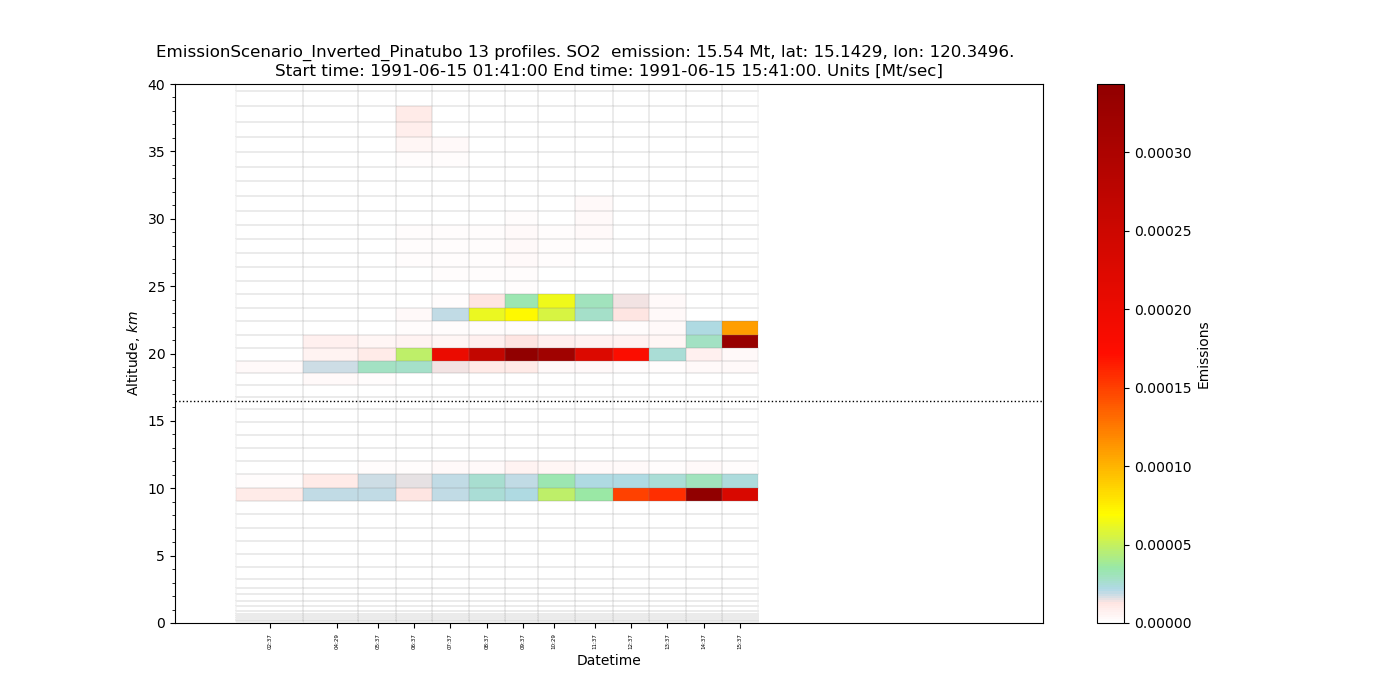
\includegraphics[width=1\linewidth]{fig3_so2_scenario_pinatubo_before.png}
    \caption{Inverted SO2 emission scenario for Mt. Pinatubo eruption in 1991 [1]. Before the remapping.}
    \label{fig3}
\end{figure}

Figure \ref{fig4} shows the same emission scenario but temporally and vertically remapped, i.e., 85 vertical profiles with uniform emission duration equal to 10 minutes.

\begin{figure}
    \centering
    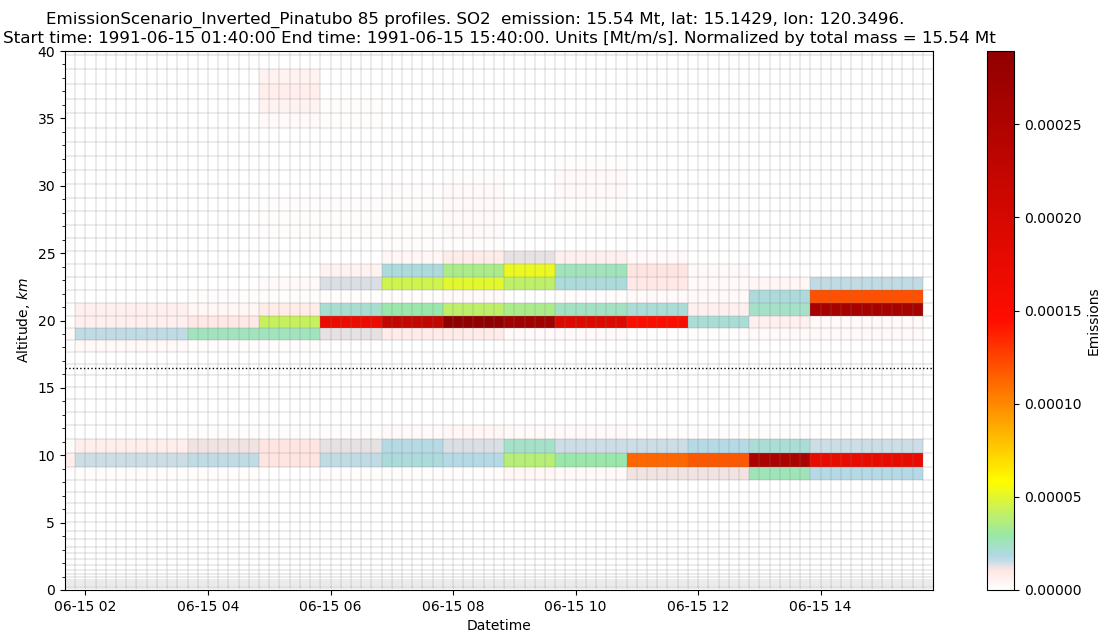
\includegraphics[width=1\linewidth]{fig4_so2_scenario_pinatubo_after.png}
    \caption{Inverted SO2 emission scenario for Mt. Pinatubo eruption in 1991 [1]. After the remapping.}
    \label{fig4}
\end{figure}

\clearpage
\subsection{WRFNetCDFWriter}
A class for writing emission data to NetCDF files compatible with the WRF-Chem model. Requires path to the 'wrfinput\_d01' file to replicate spatial dimensions for the resulting emissions 'wrfchemv\_d01' file. A visualization of the accumulated erupted mass over time is presented in Figure \ref{fig5}.

\begin{figure}
    \centering
    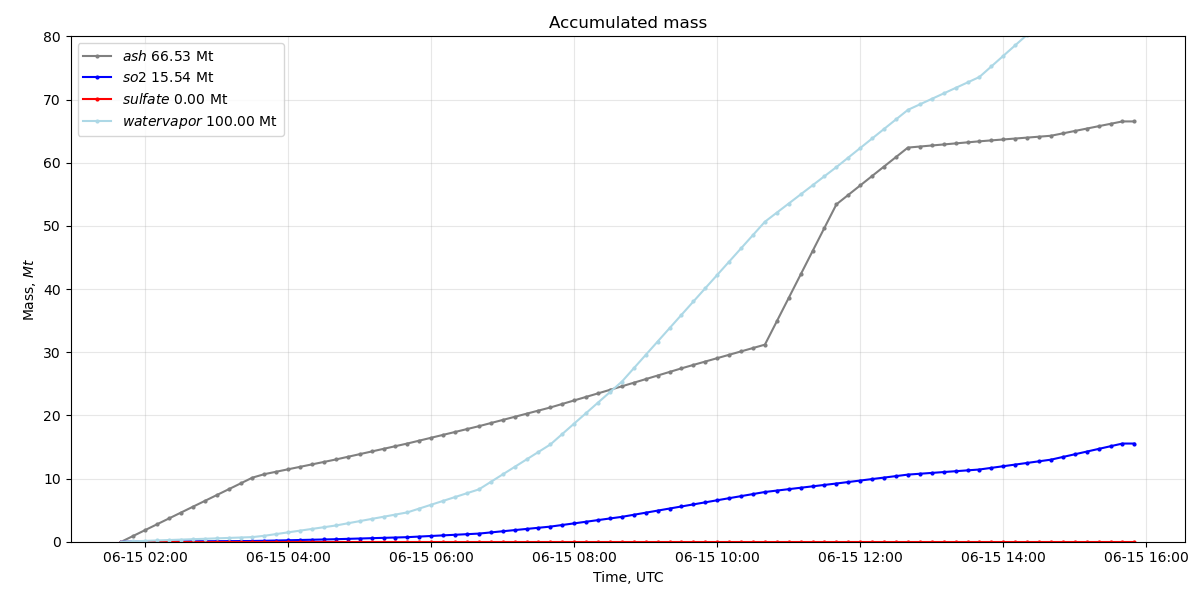
\includegraphics[width=1\linewidth]{fig5_accumulated.png}
    \caption{Distribution of accumulated mass of ash, SO2, sulfate, and water vapor for Mt. Pinatubo eruption.}
    \label{fig5}
\end{figure}


\subsection{EmissionWriter}
A class for writing emission scenarios to the emission file. Contains the abstract method 'write', which has to be overridden in child classes. Comprises scenarios and WRFNetCDFWriter instances needed to write emission data to a NetCDF file, see Figure \ref{fig1}. Child classes are the following:

\subsubsection{EmissionWriter\_UniformInTimeProfiles}
This class handles emission scenarios with uniform time intervals between profiles. No interpolation of the profiles in time and height, see example1.py and example3.py.


\subsubsection{EmissionWriter\_NonUniformInTimeHeightProfiles}
A class for handling emission scenarios with non-uniform time intervals between profiles; vertical interpolation is also implemented. See example2.py for details.

\subsubsection{EmissionWriter\_NonUniformInHeightProfiles}
This class is used to interpolate profile vertical distribution to the vertical grid from the 'wrfinput\_d01' file, see example4.py. No time interpolation, as time intervals between profiles are already uniform.


\clearpage
\section{References}
[1] Ukhov, A., Stenchikov, G., Osipov, S., Krotkov, N., Gorkavyi, N., Li, C., et al. (2023). Inverse modeling of the initial stage of the 1991 Pinatubo volcanic cloud accounting for radiative feedback of volcanic ash. Journal of Geophysical Research: Atmospheres, 128, e2022JD038446. https://doi.org/10.1029/2022JD038446.

[2] Brodtkorb, A. R., Benedictow, A., Klein, H., Kylling, A., Nyiri, A., Valdebenito, A., Sollum, E., and Kristiansen, N.: Estimating volcanic ash emissions using retrieved satellite ash columns and inverse ash transport modeling using VolcanicAshInversion v1.2.1, within the operational eEMEP (emergency European Monitoring and Evaluation Programme) volcanic plume forecasting system (version rv4_17), Geosci. Model Dev., 17, 1957–1974, https://doi.org/10.5194/gmd-17-1957-2024, 2024.

[3] Suzuki, Takeo. "A theoretical model for dispersion of tephra." Arc volcanism: physics and tectonics 95 (1983): 113.

[4] Mastin, Larry G., and Alexa R. Van Eaton. "Comparing simulations of umbrella-cloud growth and ash transport with observations from Pinatubo, Kelud, and Calbuco volcanoes." Atmosphere 11.10 (2020): 1038.


\end{document}
